% !TeX root = ../main.tex

\section{Messungen Winkel}
\label{sec:measurements-dezibot-angle}

Um die in \autoref{tab:measurements-dezibot-angle} aufgelisteten Werte so genau wie möglich zu messen, wurde ein eigenes 3D\hyphen gedrucktes Modell~\cite{felttipDezibotAlignmentPointer2025} entworfen. Dies vereinfacht das Ablesen der Winkel und verstärkt die Präzision. Weiterhin wurde ein Winkelmesser\footnote{\url{https://github.com/embedded-chess/misc/blob/main/src/protractor.pdf}} entworfen und gedruckt, auf die die Position des messendenden Dezibots sowie des Beacons inkl. Ausrichtung festgehalten ist. Durch das Fadenkreuz und den Pfeil des 3D-Modells können Messungenauigkeiten verringert werden.

Die gemessenen Rohdaten (einzelne Sensorwerte sowie Winkel) können auf GitHub\footnote{\url{https://github.com/embedded-chess/misc/blob/main/src/angle_determination_adjustment/angle_measurements.csv}} eingesehen werden. Die Winkel sind in \autoref{tab:measurements-dezibot-angle} tabellarisch sowie in \autoref{fig:measurements-dezibot-angle} grafisch dargestellt. Außerdem sind die Differenzen $\Delta\alpha$ sind in \autoref{fig:ir-signal-diff} grafisch aufbereitet.

\begin{table}[h!]
    \centering
    \begin{tabular}{cc}
    \begin{minipage}{0.3\linewidth}
        \begin{tabular}{r|rr}
            $\alpha_r$ & $\alpha_m$ & $\Delta\alpha$ \\ \hline
            0°   & 356° & -4°  \\
            10°  & 5°   & -5°  \\
            20°  & 11°  & -9°  \\
            30°  & 22°  & -8°  \\
            40°  & 30°  & -10° \\
            50°  & 41°  & -9°  \\
            60°  & 59°  & -1°  \\
            70°  & 79°  & 9°   \\
            80°  & 87°  & 7°   \\
            90°  & 93°  & 3°   \\
            100° & 98°  & -2°  \\
            110° & 106° & -4°  \\
            120° & 119° & -1°  \\
            130° & 129° & -1°  \\
            140° & 137° & -3°  \\
            150° & 149° & -1°  \\
            160° & 163° & 3°   \\
            170° & 171° & 1°   \\
        \end{tabular}
    \end{minipage}
    &
    \begin{minipage}{0.3\linewidth}
        \begin{tabular}{r|rr}
            $\alpha_r$ & $\alpha_m$ & $\Delta\alpha$ \\ \hline
            180° & 178° & -2° \\
            190° & 183° & -7° \\
            200° & 192° & -8° \\
            210° & 208° & -2° \\
            220° & 211° & -9° \\
            230° & 230° & 0°  \\
            240° & 239° & -1° \\
            250° & 250° & 0°  \\
            260° & 266° & 6°  \\
            270° & 272° & 2°  \\
            280° & 277° & -3° \\
            290° & 284° & -6° \\
            300° & 296° & -4° \\
            310° & 304° & -6° \\
            320° & 315° & -5° \\
            330° & 324° & -6° \\
            340° & 338° & -2° \\
            350° & 348° & -2° \\
        \end{tabular}
    \end{minipage}
\end{tabular}

    \caption{Signal-Messungen von \texttt{ECP\-Signal\-Detection::measure\-Dezibot\-Angle} (vgl. \autoref{sec:angle-determination}). $\alpha_r$ ist realer Winkel, in dem Dezibot in Relation zum Beacon steht. $\alpha_m$ ist Winkel, welcher vom Dezibot gemessen wurde. Daraus folgt $\Delta\alpha=\alpha_m - \alpha_r$.}
    \label{tab:measurements-dezibot-angle}
\end{table}

\begin{figure}[h]
    \centering
    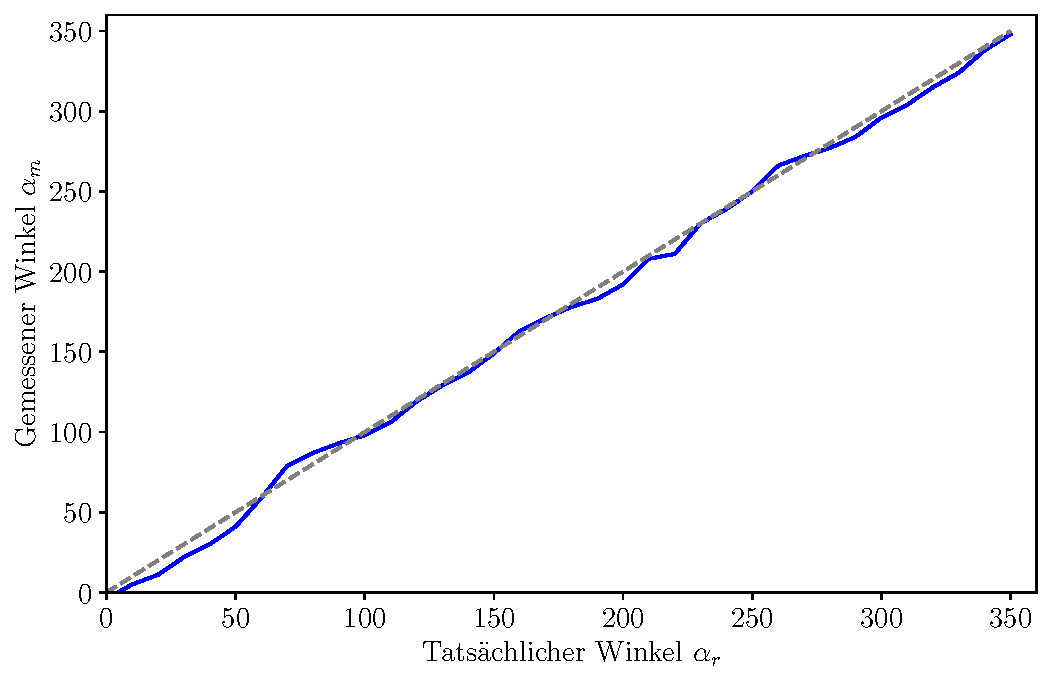
\includegraphics[width=\textwidth]{../plot/ir_signal_comparison.pdf}
    \caption{Darstellung der Daten aus \autoref{tab:measurements-dezibot-angle}.}
    \label{fig:measurements-dezibot-angle}
\end{figure}


\section{Messungen Infrarot-Rotation}
\label{sec:measurements-ir-rotation}

\begin{table}[h!]
    \centering
    \begin{tabular}{r||rrr||rrr}
    & \multicolumn{3}{c||}{Links} & \multicolumn{3}{c}{Rechts} \\ \hline
    $\alpha_{\text{initial}}$ & $\alpha_{\text{goal}}$ & $\alpha_{\text{end}}$ & $\Delta\alpha$ & $\alpha_{\text{goal}}$ & $\alpha_{\text{end}}$ & $\Delta\alpha$\\ \hline
    %
    0°   & 270°   & 260°    & 10°   & 90°   & 80°  & 10°  \\
    0°   & 270°   & 260°    & 10°   & 90°   & 75°  & 15°  \\
    0°   & 270°   & 262°    & 8°    & 90°   & 75°  & 15°  \\
    0°   & 270°   & 262°    & 8°    & 90°   & 72°  & 18°  \\
    0°   & 270°   & 260°    & 10°   & 90°   & 72°  & 18°  \\ \hline
    %
    90°  & 0°     & 5°      &-5°    & 180°  & 182° & -2°  \\
    90°  & 0°     & 10°     &-10°   & 180°  & 178° & 2°   \\
    90°  & 0°     & 12°     &-12°   & 180°  & 175° & 5°   \\
    90°  & 0°     & 10°     &-10°   & 180°  & 175° & 5°   \\
    90°  & 0°     & 8°      &-8°    & 180°  & 178° & 2°   \\ \hline
    %
    180° & 90°    & 88°    & 2°     & 270°  & 260°  & 10° \\
    180° & 90°    & 89°    & 1°     & 270°  & 260°  & 10° \\
    180° & 90°    & 92°    & -2°    & 270°  & 265°  & 5°  \\
    180° & 90°    & 88°    & 2°     & 270°  & 265°  & 5°  \\
    180° & 90°    & 88°    & 2°     & 270°  & 262°  & 8°  \\ \hline
    %
    270° & 180°   & 182°   & -2°    & 0°    & 10°   & -10° \\
    270° & 180°   & 180°   & 0°     & 0°    & 10°   & -10° \\
    270° & 180°   & 178°   & 2°     & 0°    & 10°   & -10° \\
    270° & 180°   & 182°   & -2°    & 0°    & 10°   & -10° \\
    270° & 180°   & 178°   & 2°     & 0°    & 12°   & -12°
\end{tabular}

    \caption{Messungen der Infrarot-basierten Rotation (vgl. \autoref{sec:movement-ir}). $\varphi_{\text{initial}}$: initialer Winkel, in dem Dezibot ausgerichtet ist. $\varphi_{\text{goal}}$: Ziel-Winkel, in dem Dezibot nach erfolgreicher Rotation ausgerichtet sein sollte. $\varphi_{\text{end}}$: Winkel, in dem Dezibot nach Rotation tatsächlich ausgerichtet war. $\Delta\varphi = \vert\varphi_{\text{end}}-\varphi_{\text{goal}}\vert$.}
    \label{tab:measurements-ir-rotation}
\end{table}


\section{Anpassung der Winkel-Trigonometrie}
\label{sec:angle-determination-adjustment}

Im folgenden Abschnitt soll der Ansatz zur Anpassung der Trigonometrie, welche zur Bestimmung des Signal\hyphen Winkels (vgl. \autoref{sec:angle-determination}) verwendet werden könnte, kurz beleuchtet werden.

Insgesamt ist aus \autoref{fig:angle-determination-adjustment} ersichtlich, dass die Nord- und Süd\hyphen Sensoren nicht auf der $y$-Achse liegen, sondern um 10° bzw. 28° verschoben sind. Daher sollen die Vektoren so transformiert werden, dass sie so scheinen, als würden sie aus der entsprechenden Richtung kommen.

\begin{figure}[h]
    \centering
    \begin{subfigure}[c]{0.6\textwidth}
        \centering
        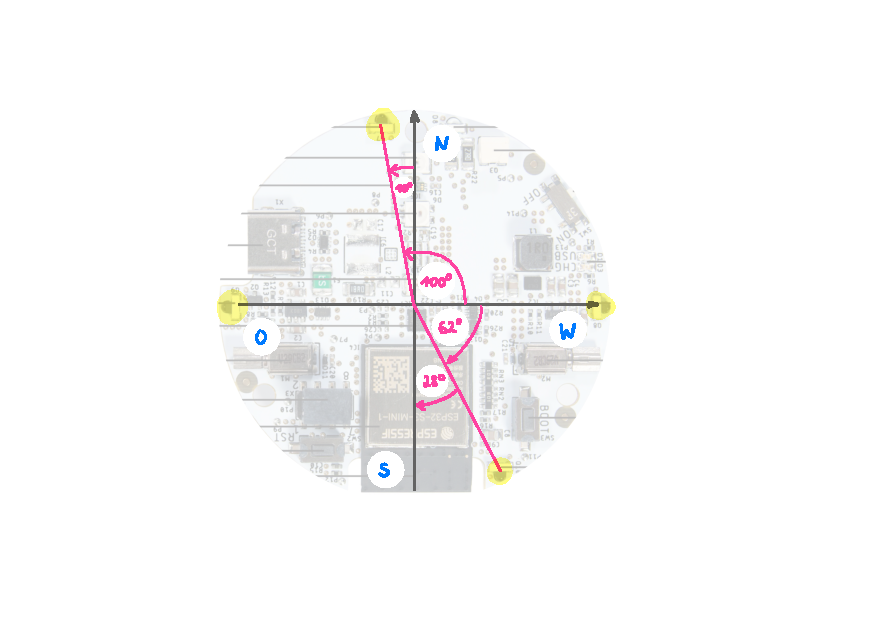
\includegraphics[width=\textwidth]{../assets/angle_determination_adjustment.pdf}
    \end{subfigure}
    \begin{subfigure}[c]{0.3\textwidth}
        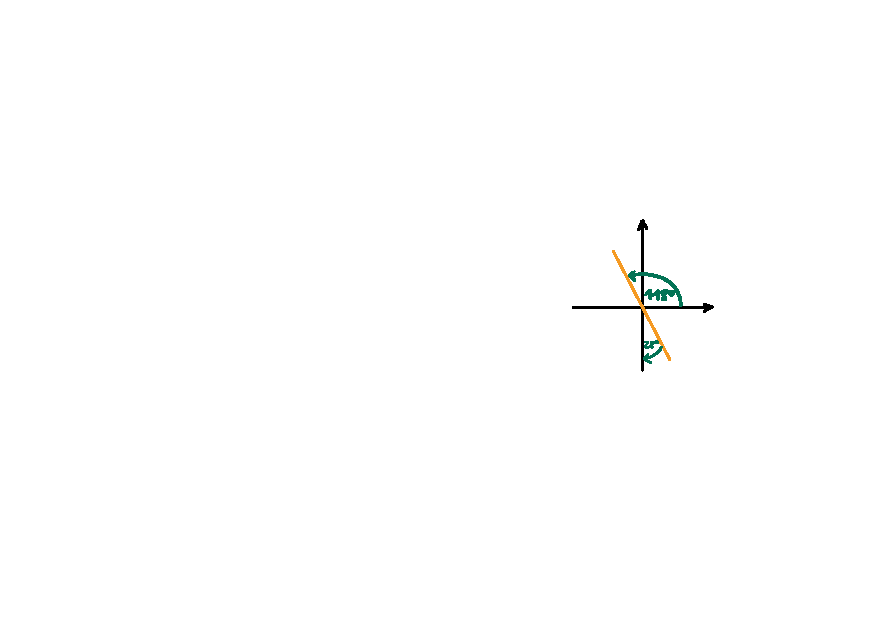
\includegraphics[width=\textwidth]{../assets/angle_determination_adjustment_south_angle.pdf}
    \end{subfigure}
    \caption{Links: Darstellung der Transformation der Nord- und Südsignale sowie der Winkel. In gelb sind die Infrarot\hyphen Sensoren hervorgehoben. Rechts: Verlängerte Funktion des Südsignals zur Bestimmung des Winkels zur $x$-Achse zur weiteren Berechnung.}
    \label{fig:angle-determination-adjustment}
\end{figure}

Daher werden die beiden Funktionen $f_n(x)=m_n\cdot x$ und $f_s(x)=m_s\cdot x$ für die Richtung der Nord- bzw. Süd\hyphen Signale aufgestellt, auf der die transformierten Werte liegen sollen. Da der Winkel zur $x$-Achse in der Rechnung verwendet wird, dürfen nicht 28° für das Süd-Signal verwendet werden, sondern der Winkel der verlängerten Funktion, d.h. 118° (siehe \autoref{fig:angle-determination-adjustment} rechts). Insgesamt ergeben sich somit folgende Anstiege und Funktionen:

\vspace{-1cm}
\begin{gather*}
    m_n = \tan(100\degree) \approx -5,671 \implies f_n(x) = -5,671x \\
    m_s = \tan(118\degree) \approx -2,901 \implies f_s(x) = -2,901x
\end{gather*}
\vspace{-1cm}

Die Distanz der Punkte, die die ursprünglichen Messwerte $n$ bzw. $s$ repräsentieren, $N=(0,n)$ bzw. $S=(0,-s)$ zum Koordinatenursprung, d.h. der Mitte des Dezibots, sei nun $d$. Die Distanz soll nach der Transformation erhalten bleiben, um die Stärke des Signals nicht zu verfälschen. Somit ergeben sich folgende Überlegung zur Bestimmung der transformierten Punkte.

\begin{gather*}
    ~\\[-1.25cm]
    \begin{aligned}
        d^2 &= x^2 + y^2 \\
        \implies d &= \sqrt{x^2 + y^2} = \sqrt{x^2 + f(x)^2} = \sqrt{x^2 + (mx)^2} \\
        \implies d &= \sqrt{x^2 (1 + m^2)} = |x| \cdot \sqrt{1+m^2} \\
        \implies |x| &= \frac{d}{\sqrt{1+m^2}} \\
        \implies x_{1,2} &= \pm \frac{d}{\sqrt{1+m^2}} \\
        \implies f(x_1) &= \underbrace{+ \frac{d}{\sqrt{1+m^2}}}_{=~x_1} \cdot m, \quad
    f(x_2) = \underbrace{- \frac{d}{\sqrt{1+m^2}}}_{=~x_2} \cdot m \\
    \end{aligned} \\
    %
    \implies P_1=\left(+ \frac{d}{\sqrt{1+m^2}}; + \frac{dm}{\sqrt{1+m^2}}\right), \quad
    P_2=\left(-\frac{d}{\sqrt{1+m^2}}; -\frac{dm}{\sqrt{1+m^2}}\right)
\end{gather*}
\vspace{-0.5cm}

Insgesamt ergeben sich zwei mögliche Lösungen $P_1$ und $P_2$. Aufgrund der Anordnung von Nord und Süd folgt:

\vspace{-0.75cm}
\begin{gather*}
    \begin{aligned}
        N' &\approx \left(-\frac{n}{\sqrt{1+(-5,6713)^2}}; -\frac{-5,6713n}{\sqrt{1+(-5,6713)^2}}\right) \approx \left(-0,174n; 0,985n\right) \\[0.2cm]
        %
        S' &\approx \left(+ \frac{s}{\sqrt{1+(-2,901)^2}}; + \frac{-2,901s}{\sqrt{1+(-2,901)^2}}\right) \approx \left( 0,469s; -0,883s \right)
    \end{aligned}
\end{gather*}
\vspace{-0.5cm}

Ein Beispiel für die Transformation ist in \autoref{fig:angle-determination-adjustment-example} dargestellt.

\begin{figure}[h]
    \centering
    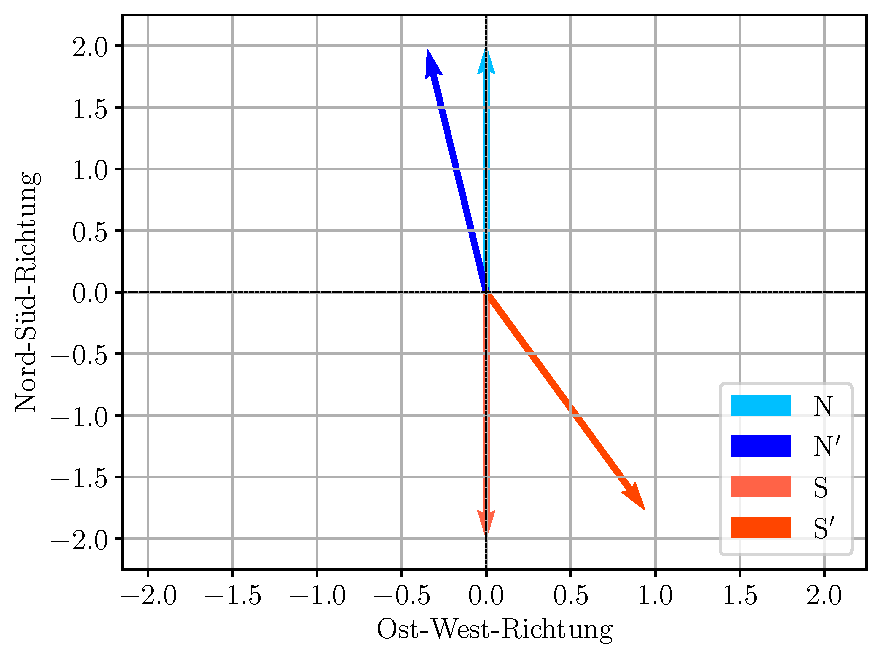
\includegraphics[width=\textwidth]{../plot/angle_adjustment/trigonometry.pdf}
    \caption{Beispiel für die Transformation vom ursprünglichen Nord- $N$ und Süd\hyphen Signal $S'$ zu $N'$ bzw $S'$.}
    \label{fig:angle-determination-adjustment-example}
\end{figure}

Zur Berechnung der Winkel muss das Verfahren zur Berechnung der Resultanten aus \autoref{sec:angle-determination} wie folgt angepasst werden:

\vspace{-0.75cm}
\begin{gather*}
    \begin{aligned}
        r_x &= -0,174n + e + 0,469s - w \\
        r_y &= 0,985n - 0,883s
    \end{aligned}
\end{gather*}
\vspace{-0.5cm}

Eine Beispiel\hyphen Rechnung sieht wie folgt aus:

\vspace{-0.75cm}
\begin{gather*}
    n=0,5, ~e=0,2, ~s=0,2, ~w=1,0  \\
    \begin{aligned}
        \text{alt:}~~ &R = \begin{pmatrix} 0,8000 \\ 0,3000 \end{pmatrix} &\Rightarrow \varphi=291\degree \\
        \text{neu:}~~ &R = \begin{pmatrix} -0,7928 \\ 0,3158 \end{pmatrix} &\Rightarrow \varphi=292\degree
    \end{aligned}
\end{gather*}
\vspace{-0.5cm}

Beim Testen fiel jedoch auf, dass der Ansatz keine große Verbesserung brachte. Die Differenz zu den tatsächlichen Werten schwankte nun teilweise weitaus mehr -- bis zu 30° bei Ausrichtung nach Süden. Dies ist nachvollziehbar, da die Infrarot\hyphen Sensoren nicht in die transformierte Richtung ausgerichtet sind, sonder nur verschoben. Daher wurde dieser Ansatz verworfen.
